\pagebreak
\section{Problemy}

\begin{figure}
	\centering
	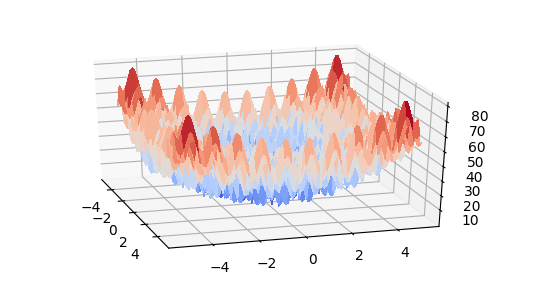
\includegraphics[width=\linewidth]{imgs/rastrigin_plot}
	\caption{Funkcja testowa.}
	\label{fig:rastrigin_plot}
\end{figure}

%2. Problemy
%- problem funkcji (rastrigin dla 2D danych, zrzut ekranu/ 3D, zakres wartości, minimalizacja itp.)
%- problem pokoju (planowanie, jakie meble, jak przebiega ocena - pseudokod funkcji eval_room)
%
%3. Algorytmy:
%- 3 algorytmy (PSO, FFA, BAT)
%- jakie ogólne parametry (liczba osobników, zakres wartości, liczba wymiarów)
%- dla każdego alg. jakie parametry (jakie i co oznaczają)
%
%4. Wyniki:
%- odpalić każdy z alg. dla każdego problemu z 3-5 razy
%- przykładowe screeny GUI
%- aggregacje kilku uruchomień
%[bardziej zrób placeholdery]
%
%5. Wnioski:
%[placeholder]